\documentclass[xcolor=dvipanames]{beamer}
\usetheme{Madrid}

\usepackage{listings} % for displaying code

\title{Anki-Pdf-Editor}
\subtitle{Javafx + Spring}
\author{derMacon}

% to make a list of frames possible: 
% https://tex.stackexchange.com/questions/56512/is-there-any-way-to-produce-list-of-frames-with-beamer
\makeatletter
\newcommand\listofframes{\@starttoc{lbf}}
\makeatother
\addtobeamertemplate{frametitle}{}{%
  \addcontentsline{lbf}{section}{\protect\makebox[2em][l]{%
    \protect\usebeamercolor[fg]{structure}\textbullet\hfill}%
  \insertframetitle\par}%
}

\begin{document}
	\begin{frame}
		\titlepage
	\end{frame}
	
	\begin{frame}
		\listofframes
	\end{frame}
		
	\begin{frame}
		\frametitle{Introduction}
		Commandline tool to create anki flash cards via the vim editor. Once started the programm will display a selected pdf document in which the user can navigate throughout vim itself. If a anki-card should contain a specific pdf page of the displayed document on either the front- or the backside of a note it can be passed in a simplyfied version where the pagenumber is written between tags.

All features can be used via shortcuts. For that the program opens a costum .vimrc.
	\end{frame}
	
	\begin{frame}
		\frametitle{Installation / Requirements}
		\begin{itemize}
			\item Unix OS (due to filepaths)
			\item Vim
			\item Ankidroid 2.1 (or newer)
			\item Ankiconnect addon 
			\item gnome-terminal (terminal emulation)
		\end{itemize}
	\end{frame}
	
	\begin{frame}	
	\begin{columns}

		\column{0.5\textwidth}
	
		\frametitle{Usage}
		\begin{itemize}
			\item To open run the programm run the command `java -jar \emph{path/to/jar}`. Once run, spring will allocate the 8080 port on the machine and expose a rest api.
		
			\item The user will be confronted with the following menu:			
		\end{itemize}	
		
		
		\column{0.5\textwidth}	
			\begin{figure}
			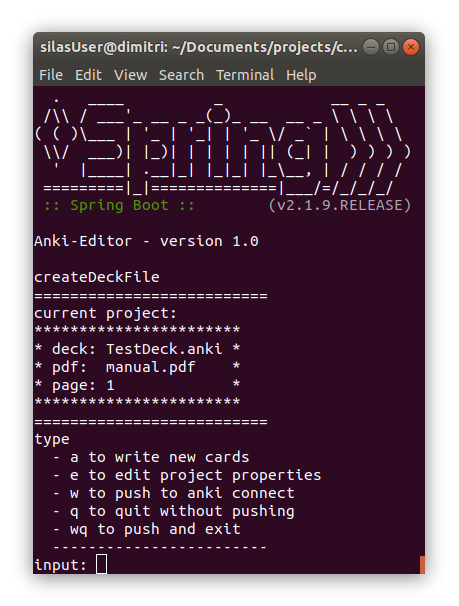
\includegraphics[scale=0.35]{./img/topLevelMenu.png}
			\caption{top level menu}
			\end{figure}
			
	\end{columns}
	\end{frame}
	
	\begin{frame}
		\frametitle{Edit project properties}
		\begin{columns}
			\column{0.5\textwidth}	
				\begin{itemize}
					\item{When selecting the project properties the user has the choice to either change the displayed pdf or the stack of cards to which the cards should be added}
				\end{itemize}
			
			\column{0.5\textwidth}	
				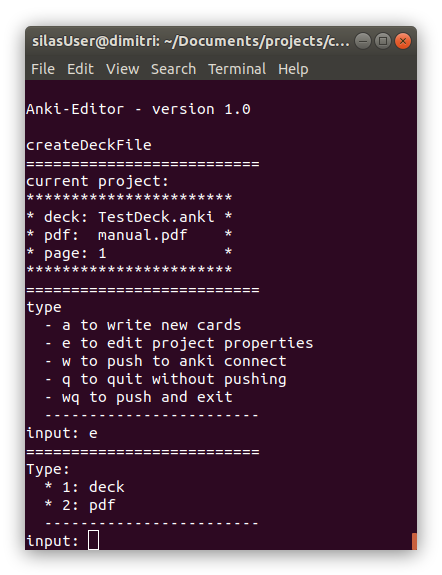
\includegraphics[scale=.35]{./img/editProperties_menu.png}
		\end{columns}
	\end{frame}
	
	\begin{frame}
		\begin{center}
			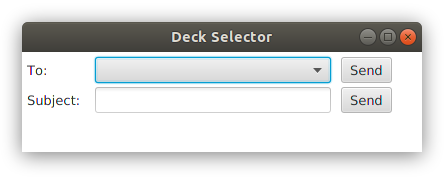
\includegraphics[scale=.35]{./img/editProperties_deckSelection.png}
			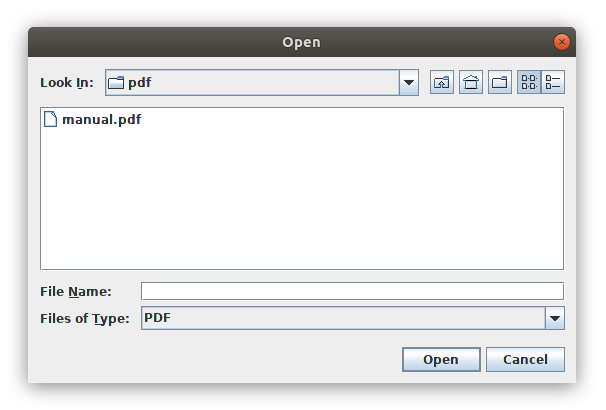
\includegraphics[scale=.35]{./img/editProperties_pdfSelection.png}
		\end{center}
	\end{frame}
	
	
	\begin{frame}
		\frametitle{Creating new cards}
		\begin{itemize}
			\item a javafx gui will load containing a pdf viewer showing the selected pdf
			\item a second window containing a vim instance will open. This vim session is capable of communicating with the exposed rest api. By pressing either \emph{z} (next page) or \emph{shift + z} (previous page) the pdf viewer updates accordingly. 
			\item to import / paste the displayed image as a png in the current card just press \emph{p} and an image tag with the following syntax will be pasted into the document at the cursor position: \emph{<PDF_PAGE_NUM>}
			\item if the user has overwritten this register the page is also accessable via the keykombination \emph{,p}
		\end{itemize}
	\end{frame}
	
	\begin{frame}
		\frametitle{Parsing user content}
		\begin{itemize}
			\item to parse the user input to actual anki cards the user has to save his written content via \emph{:wq} in the vim instance and type \emph{alt + f4} to exit pdf viewer. 
			\item in the top level menu either select \emph{w} or \emph{wq}
			\item in the background the java backend will generate the required json format for the ankidroid api (AnkiConnect)
			\item the json also contains html elements for the given images / linebreaks to ensure a readable anki card 
			\item after pushing the changes to the anki rest api, the cards should be displayed in the appropriate deck in the anki desktop program itself.
		\end{itemize}
	\end{frame}
	
	\begin{frame}
		\frametitle{Shortcuts - Programm specific}
		All program specific shortcuts in a nutshell: 
		\begin{itemize}
			\item \emph{z} / \emph{shift + z}: turn next / previous page; Copy the current page tag to the default register (accessed via \emph{p})
			\item \emph{, + c}: Append new card template to anki file
			\item \emph{,+ p}: Reload page tag, pastes the current page tag to cursor position
			\item \emph{, + t} / \emph{, + shift + t}: tab between fields
		\end{itemize}
	\end{frame}
	
	\begin{frame}
		\frametitle{Shortcuts - Vim in general}
		\begin{center}
			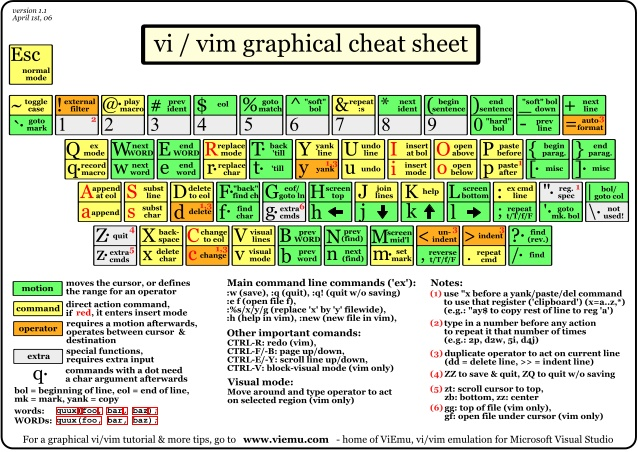
\includegraphics[scale=.48]{./img/vim-cheat-sheet.jpg}
		\end{center}
	\end{frame}
		
	
	
\end{document}
